\documentclass[1p]{elsarticle_modified}
%\bibliographystyle{elsarticle-num}

%\usepackage[colorlinks]{hyperref}
%\usepackage{abbrmath_seonhwa} %\Abb, \Ascr, \Acal ,\Abf, \Afrak
\usepackage{amsfonts}
\usepackage{amssymb}
\usepackage{amsmath}
\usepackage{amsthm}
\usepackage{scalefnt}
\usepackage{amsbsy}
\usepackage{kotex}
\usepackage{caption}
\usepackage{subfig}
\usepackage{color}
\usepackage{graphicx}
\usepackage{xcolor} %% white, black, red, green, blue, cyan, magenta, yellow
\usepackage{float}
\usepackage{setspace}
\usepackage{hyperref}

\usepackage{tikz}
\usetikzlibrary{arrows}

\usepackage{multirow}
\usepackage{array} % fixed length table
\usepackage{hhline}

%%%%%%%%%%%%%%%%%%%%%
\makeatletter
\renewcommand*\env@matrix[1][\arraystretch]{%
	\edef\arraystretch{#1}%
	\hskip -\arraycolsep
	\let\@ifnextchar\new@ifnextchar
	\array{*\c@MaxMatrixCols c}}
\makeatother %https://tex.stackexchange.com/questions/14071/how-can-i-increase-the-line-spacing-in-a-matrix
%%%%%%%%%%%%%%%

\usepackage[normalem]{ulem}

\newcommand{\msout}[1]{\ifmmode\text{\sout{\ensuremath{#1}}}\else\sout{#1}\fi}
%SOURCE: \msout is \stkout macro in https://tex.stackexchange.com/questions/20609/strikeout-in-math-mode

\newcommand{\cancel}[1]{
	\ifmmode
	{\color{red}\msout{#1}}
	\else
	{\color{red}\sout{#1}}
	\fi
}

\newcommand{\add}[1]{
	{\color{blue}\uwave{#1}}
}

\newcommand{\replace}[2]{
	\ifmmode
	{\color{red}\msout{#1}}{\color{blue}\uwave{#2}}
	\else
	{\color{red}\sout{#1}}{\color{blue}\uwave{#2}}
	\fi
}

\newcommand{\Sol}{\mathcal{S}} %segment
\newcommand{\D}{D} %diagram
\newcommand{\A}{\mathcal{A}} %arc


%%%%%%%%%%%%%%%%%%%%%%%%%%%%%5 test

\def\sl{\operatorname{\textup{SL}}(2,\Cbb)}
\def\psl{\operatorname{\textup{PSL}}(2,\Cbb)}
\def\quan{\mkern 1mu \triangleright \mkern 1mu}

\theoremstyle{definition}
\newtheorem{thm}{Theorem}[section]
\newtheorem{prop}[thm]{Proposition}
\newtheorem{lem}[thm]{Lemma}
\newtheorem{ques}[thm]{Question}
\newtheorem{cor}[thm]{Corollary}
\newtheorem{defn}[thm]{Definition}
\newtheorem{exam}[thm]{Example}
\newtheorem{rmk}[thm]{Remark}
\newtheorem{alg}[thm]{Algorithm}

\newcommand{\I}{\sqrt{-1}}
\begin{document}

%\begin{frontmatter}
%
%\title{Boundary parabolic representations of knots up to 8 crossings}
%
%%% Group authors per affiliation:
%\author{Yunhi Cho} 
%\address{Department of Mathematics, University of Seoul, Seoul, Korea}
%\ead{yhcho@uos.ac.kr}
%
%
%\author{Seonhwa Kim} %\fnref{s_kim}}
%\address{Center for Geometry and Physics, Institute for Basic Science, Pohang, 37673, Korea}
%\ead{ryeona17@ibs.re.kr}
%
%\author{Hyuk Kim}
%\address{Department of Mathematical Sciences, Seoul National University, Seoul 08826, Korea}
%\ead{hyukkim@snu.ac.kr}
%
%\author{Seokbeom Yoon}
%\address{Department of Mathematical Sciences, Seoul National University, Seoul, 08826,  Korea}
%\ead{sbyoon15@snu.ac.kr}
%
%\begin{abstract}
%We find all boundary parabolic representation of knots up to 8 crossings.
%
%\end{abstract}
%\begin{keyword}
%    \MSC[2010] 57M25 
%\end{keyword}
%
%\end{frontmatter}

%\linenumbers
%\tableofcontents
%
\newcommand\colored[1]{\textcolor{white}{\rule[-0.35ex]{0.8em}{1.4ex}}\kern-0.8em\color{red} #1}%
%\newcommand\colored[1]{\textcolor{white}{ #1}\kern-2.17ex	\textcolor{white}{ #1}\kern-1.81ex	\textcolor{white}{ #1}\kern-2.15ex\color{red}#1	}

{\Large $\underline{12a_{0813}~(K12a_{0813})}$}

\setlength{\tabcolsep}{10pt}
\renewcommand{\arraystretch}{1.6}
\vspace{1cm}\begin{tabular}{m{100pt}>{\centering\arraybackslash}m{274pt}}
\multirow{5}{120pt}{
	\centering
	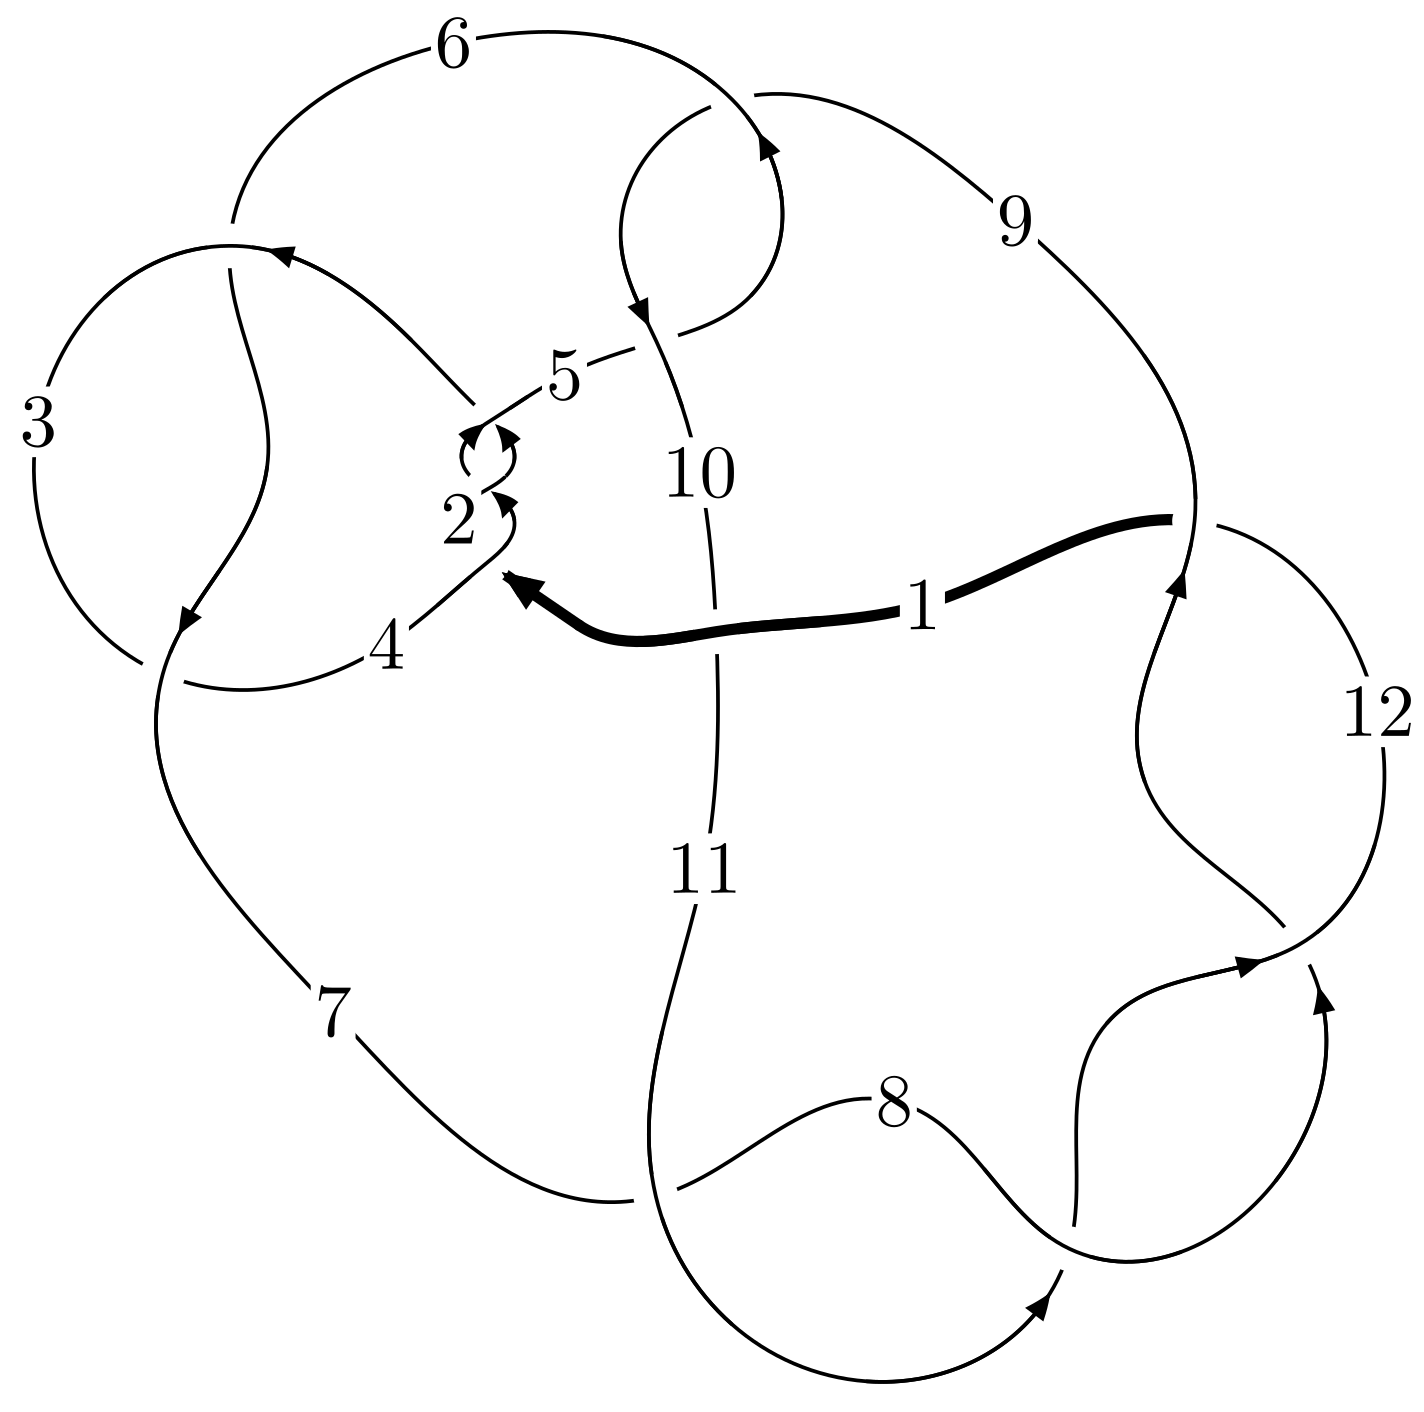
\includegraphics[width=112pt]{../../../GIT/diagram.site/Diagrams/png/1614_12a_0813.png}\\
\ \ \ A knot diagram\footnotemark}&
\allowdisplaybreaks
\textbf{Linearized knot diagam} \\
\cline{2-2}
 &
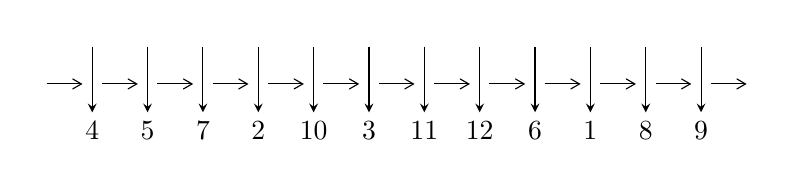
\begin{tikzpicture}[x=20pt, y=17pt]
	% nodes
	\node (C0) at (0, 0) {};
	\node (C1) at (1, 0) {};
	\node (C1U) at (1, +1) {};
	\node (C1D) at (1, -1) {4};

	\node (C2) at (2, 0) {};
	\node (C2U) at (2, +1) {};
	\node (C2D) at (2, -1) {5};

	\node (C3) at (3, 0) {};
	\node (C3U) at (3, +1) {};
	\node (C3D) at (3, -1) {7};

	\node (C4) at (4, 0) {};
	\node (C4U) at (4, +1) {};
	\node (C4D) at (4, -1) {2};

	\node (C5) at (5, 0) {};
	\node (C5U) at (5, +1) {};
	\node (C5D) at (5, -1) {10};

	\node (C6) at (6, 0) {};
	\node (C6U) at (6, +1) {};
	\node (C6D) at (6, -1) {3};

	\node (C7) at (7, 0) {};
	\node (C7U) at (7, +1) {};
	\node (C7D) at (7, -1) {11};

	\node (C8) at (8, 0) {};
	\node (C8U) at (8, +1) {};
	\node (C8D) at (8, -1) {12};

	\node (C9) at (9, 0) {};
	\node (C9U) at (9, +1) {};
	\node (C9D) at (9, -1) {6};

	\node (C10) at (10, 0) {};
	\node (C10U) at (10, +1) {};
	\node (C10D) at (10, -1) {1};

	\node (C11) at (11, 0) {};
	\node (C11U) at (11, +1) {};
	\node (C11D) at (11, -1) {8};

	\node (C12) at (12, 0) {};
	\node (C12U) at (12, +1) {};
	\node (C12D) at (12, -1) {9};
	\node (C13) at (13, 0) {};

	% arrows
	\draw[->,>={angle 60}]
	(C0) edge (C1) (C1) edge (C2) (C2) edge (C3) (C3) edge (C4) (C4) edge (C5) (C5) edge (C6) (C6) edge (C7) (C7) edge (C8) (C8) edge (C9) (C9) edge (C10) (C10) edge (C11) (C11) edge (C12) (C12) edge (C13) ;	\draw[->,>=stealth]
	(C1U) edge (C1D) (C2U) edge (C2D) (C3U) edge (C3D) (C4U) edge (C4D) (C5U) edge (C5D) (C6U) edge (C6D) (C7U) edge (C7D) (C8U) edge (C8D) (C9U) edge (C9D) (C10U) edge (C10D) (C11U) edge (C11D) (C12U) edge (C12D) ;
	\end{tikzpicture} \\
\hhline{~~} \\& 
\textbf{Solving Sequence} \\ \cline{2-2} 
 &
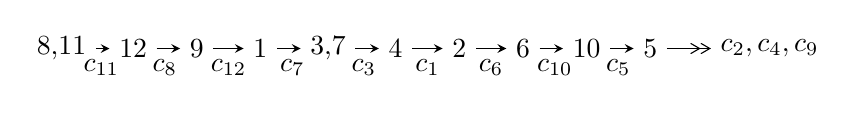
\begin{tikzpicture}[x=23pt, y=7pt]
	% node
	\node (A0) at (-1/8, 0) {8,11};
	\node (A1) at (1, 0) {12};
	\node (A2) at (2, 0) {9};
	\node (A3) at (3, 0) {1};
	\node (A4) at (65/16, 0) {3,7};
	\node (A5) at (41/8, 0) {4};
	\node (A6) at (49/8, 0) {2};
	\node (A7) at (57/8, 0) {6};
	\node (A8) at (65/8, 0) {10};
	\node (A9) at (73/8, 0) {5};
	\node (C1) at (1/2, -1) {$c_{11}$};
	\node (C2) at (3/2, -1) {$c_{8}$};
	\node (C3) at (5/2, -1) {$c_{12}$};
	\node (C4) at (7/2, -1) {$c_{7}$};
	\node (C5) at (37/8, -1) {$c_{3}$};
	\node (C6) at (45/8, -1) {$c_{1}$};
	\node (C7) at (53/8, -1) {$c_{6}$};
	\node (C8) at (61/8, -1) {$c_{10}$};
	\node (C9) at (69/8, -1) {$c_{5}$};
	\node (A10) at (11, 0) {$c_{2},c_{4},c_{9}$};

	% edge
	\draw[->,>=stealth]	
	(A0) edge (A1) (A1) edge (A2) (A2) edge (A3) (A3) edge (A4) (A4) edge (A5) (A5) edge (A6) (A6) edge (A7) (A7) edge (A8) (A8) edge (A9) ;
	\draw[->>,>={angle 60}]	
	(A9) edge (A10);
\end{tikzpicture} \\ 

\end{tabular} \\

\footnotetext{
The image of knot diagram is generated by the software ``\textbf{Draw programme}" developed by Andrew Bartholomew(\url{http://www.layer8.co.uk/maths/draw/index.htm\#Running-draw}), where we modified some parts for our purpose(\url{https://github.com/CATsTAILs/LinksPainter}).
}\phantom \\ \newline 
\centering \textbf{Ideals for irreducible components\footnotemark of $X_{\text{par}}$} 
 
\begin{align*}
I^u_{1}&=\langle 
-7.95449\times10^{20} u^{71}-4.31806\times10^{21} u^{70}+\cdots+1.48712\times10^{21} b-3.47841\times10^{21},\\
\phantom{I^u_{1}}&\phantom{= \langle  }1.07241\times10^{22} u^{71}+2.56114\times10^{22} u^{70}+\cdots+2.97424\times10^{21} a+7.95838\times10^{21},\;u^{72}+4 u^{71}+\cdots+4 u+1\rangle \\
I^u_{2}&=\langle 
u^5+u^4-3 u^3- u^2+b+2 u-2,\;u^5+u^4-3 u^3- u^2+a+2 u-2,\;u^6+u^5-3 u^4-2 u^3+2 u^2- u-1\rangle \\
I^u_{3}&=\langle 
b- u-2,\;a- u-1,\;u^2- u-1\rangle \\
I^u_{4}&=\langle 
b+u+2,\;a+2 u,\;u^2- u-1\rangle \\
\\
\end{align*}
\raggedright * 4 irreducible components of $\dim_{\mathbb{C}}=0$, with total 82 representations.\\
\footnotetext{All coefficients of polynomials are rational numbers. But the coefficients are sometimes approximated in decimal forms when there is not enough margin.}
\newpage
\renewcommand{\arraystretch}{1}
\centering \section*{I. $I^u_{1}= \langle -7.95\times10^{20} u^{71}-4.32\times10^{21} u^{70}+\cdots+1.49\times10^{21} b-3.48\times10^{21},\;1.07\times10^{22} u^{71}+2.56\times10^{22} u^{70}+\cdots+2.97\times10^{21} a+7.96\times10^{21},\;u^{72}+4 u^{71}+\cdots+4 u+1 \rangle$}
\flushleft \textbf{(i) Arc colorings}\\
\begin{tabular}{m{7pt} m{180pt} m{7pt} m{180pt} }
\flushright $a_{8}=$&$\begin{pmatrix}0\\u\end{pmatrix}$ \\
\flushright $a_{11}=$&$\begin{pmatrix}1\\0\end{pmatrix}$ \\
\flushright $a_{12}=$&$\begin{pmatrix}1\\u^2\end{pmatrix}$ \\
\flushright $a_{9}=$&$\begin{pmatrix}- u\\- u^3+u\end{pmatrix}$ \\
\flushright $a_{1}=$&$\begin{pmatrix}- u^2+1\\- u^4+2 u^2\end{pmatrix}$ \\
\flushright $a_{3}=$&$\begin{pmatrix}-3.60565 u^{71}-8.61108 u^{70}+\cdots-3.99235 u-2.67577\\0.534891 u^{71}+2.90363 u^{70}+\cdots+4.98903 u+2.33902\end{pmatrix}$ \\
\flushright $a_{7}=$&$\begin{pmatrix}u\\u\end{pmatrix}$ \\
\flushright $a_{4}=$&$\begin{pmatrix}-11.5779 u^{71}-28.0840 u^{70}+\cdots-20.0416 u-7.72322\\-7.43736 u^{71}-16.5693 u^{70}+\cdots-11.0602 u-2.70843\end{pmatrix}$ \\
\flushright $a_{2}=$&$\begin{pmatrix}16.6166 u^{71}+39.8106 u^{70}+\cdots+30.7682 u+9.88627\\14.7571 u^{71}+34.3253 u^{70}+\cdots+26.7496 u+6.90106\end{pmatrix}$ \\
\flushright $a_{6}=$&$\begin{pmatrix}-2.38563 u^{71}-6.49739 u^{70}+\cdots-5.92951 u-3.30940\\1.63521 u^{71}+4.28995 u^{70}+\cdots+4.95437 u+0.667990\end{pmatrix}$ \\
\flushright $a_{10}=$&$\begin{pmatrix}- u^6+3 u^4-2 u^2+1\\- u^8+4 u^6-4 u^4\end{pmatrix}$ \\
\flushright $a_{5}=$&$\begin{pmatrix}10.9945 u^{71}+25.9002 u^{70}+\cdots+23.1121 u+4.39475\\12.8540 u^{71}+31.3855 u^{70}+\cdots+27.1307 u+7.37996\end{pmatrix}$\\&\end{tabular}
\flushleft \textbf{(ii) Obstruction class $= -1$}\\~\\
\flushleft \textbf{(iii) Cusp Shapes $= \frac{150126529301461580621605}{2974244354519536997566} u^{71}+\frac{259807076562668316197598}{1487122177259768498783} u^{70}+\cdots+\frac{302915952567745176733616}{1487122177259768498783} u+\frac{237828014772875129379223}{2974244354519536997566}$}\\~\\
\newpage\renewcommand{\arraystretch}{1}
\flushleft \textbf{(iv) u-Polynomials at the component}\newline \\
\begin{tabular}{m{50pt}|m{274pt}}
Crossings & \hspace{64pt}u-Polynomials at each crossing \\
\hline $$\begin{aligned}c_{1},c_{2},c_{4}\end{aligned}$$&$\begin{aligned}
&u^{72}-9 u^{71}+\cdots-23 u-1
\end{aligned}$\\
\hline $$\begin{aligned}c_{3},c_{6}\end{aligned}$$&$\begin{aligned}
&u^{72}+3 u^{71}+\cdots-320 u-64
\end{aligned}$\\
\hline $$\begin{aligned}c_{5},c_{9}\end{aligned}$$&$\begin{aligned}
&u^{72}+2 u^{71}+\cdots+64 u+16
\end{aligned}$\\
\hline $$\begin{aligned}c_{7},c_{8},c_{11}\\c_{12}\end{aligned}$$&$\begin{aligned}
&u^{72}+4 u^{71}+\cdots+4 u+1
\end{aligned}$\\
\hline $$\begin{aligned}c_{10}\end{aligned}$$&$\begin{aligned}
&u^{72}-20 u^{71}+\cdots-3276 u-79
\end{aligned}$\\
\hline
\end{tabular}\\~\\
\newpage\renewcommand{\arraystretch}{1}
\flushleft \textbf{(v) Riley Polynomials at the component}\newline \\
\begin{tabular}{m{50pt}|m{274pt}}
Crossings & \hspace{64pt}Riley Polynomials at each crossing \\
\hline $$\begin{aligned}c_{1},c_{2},c_{4}\end{aligned}$$&$\begin{aligned}
&y^{72}-71 y^{71}+\cdots-369 y+1
\end{aligned}$\\
\hline $$\begin{aligned}c_{3},c_{6}\end{aligned}$$&$\begin{aligned}
&y^{72}-45 y^{71}+\cdots-241664 y+4096
\end{aligned}$\\
\hline $$\begin{aligned}c_{5},c_{9}\end{aligned}$$&$\begin{aligned}
&y^{72}+30 y^{71}+\cdots-3712 y+256
\end{aligned}$\\
\hline $$\begin{aligned}c_{7},c_{8},c_{11}\\c_{12}\end{aligned}$$&$\begin{aligned}
&y^{72}-84 y^{71}+\cdots-20 y+1
\end{aligned}$\\
\hline $$\begin{aligned}c_{10}\end{aligned}$$&$\begin{aligned}
&y^{72}-12 y^{71}+\cdots-11660268 y+6241
\end{aligned}$\\
\hline
\end{tabular}\\~\\
\newpage\flushleft \textbf{(vi) Complex Volumes and Cusp Shapes}
$$\begin{array}{c|c|c}  
\text{Solutions to }I^u_{1}& \I (\text{vol} + \sqrt{-1}CS) & \text{Cusp shape}\\
 \hline 
\begin{aligned}
u &= -0.982343 + 0.346269 I \\
a &= \phantom{-}0.216789 - 0.337856 I \\
b &= \phantom{-}1.196170 + 0.510620 I\end{aligned}
 & -7.89851 - 4.44178 I & \phantom{-0.000000 } 0 \\ \hline\begin{aligned}
u &= -0.982343 - 0.346269 I \\
a &= \phantom{-}0.216789 + 0.337856 I \\
b &= \phantom{-}1.196170 - 0.510620 I\end{aligned}
 & -7.89851 + 4.44178 I & \phantom{-0.000000 } 0 \\ \hline\begin{aligned}
u &= \phantom{-}0.757927 + 0.551621 I \\
a &= -0.323743 - 0.008309 I \\
b &= -1.90119 + 0.21928 I\end{aligned}
 & -6.15007 - 12.15710 I & \phantom{-0.000000 } 0 \\ \hline\begin{aligned}
u &= \phantom{-}0.757927 - 0.551621 I \\
a &= -0.323743 + 0.008309 I \\
b &= -1.90119 - 0.21928 I\end{aligned}
 & -6.15007 + 12.15710 I & \phantom{-0.000000 } 0 \\ \hline\begin{aligned}
u &= -0.850217 + 0.222300 I \\
a &= -0.623196 + 0.202068 I \\
b &= -1.52408 - 0.38478 I\end{aligned}
 & -2.05877 - 1.35062 I & \phantom{-0.000000 } 0 \\ \hline\begin{aligned}
u &= -0.850217 - 0.222300 I \\
a &= -0.623196 - 0.202068 I \\
b &= -1.52408 + 0.38478 I\end{aligned}
 & -2.05877 + 1.35062 I & \phantom{-0.000000 } 0 \\ \hline\begin{aligned}
u &= \phantom{-}0.705422 + 0.506721 I \\
a &= \phantom{-}0.424505 + 0.257141 I \\
b &= \phantom{-}1.87330 - 0.07115 I\end{aligned}
 & -0.21486 - 7.76434 I & \phantom{-0.000000 } 0 \\ \hline\begin{aligned}
u &= \phantom{-}0.705422 - 0.506721 I \\
a &= \phantom{-}0.424505 - 0.257141 I \\
b &= \phantom{-}1.87330 + 0.07115 I\end{aligned}
 & -0.21486 + 7.76434 I & \phantom{-0.000000 } 0 \\ \hline\begin{aligned}
u &= -0.681164 + 0.507135 I \\
a &= -0.004024 - 0.372323 I \\
b &= -1.55030 - 0.84093 I\end{aligned}
 & -8.10918 + 5.48099 I & \phantom{-0.000000 } 0 \\ \hline\begin{aligned}
u &= -0.681164 - 0.507135 I \\
a &= -0.004024 + 0.372323 I \\
b &= -1.55030 + 0.84093 I\end{aligned}
 & -8.10918 - 5.48099 I & \phantom{-0.000000 } 0\\
 \hline 
 \end{array}$$\newpage$$\begin{array}{c|c|c}  
\text{Solutions to }I^u_{1}& \I (\text{vol} + \sqrt{-1}CS) & \text{Cusp shape}\\
 \hline 
\begin{aligned}
u &= \phantom{-}0.697751 + 0.460295 I \\
a &= -0.046939 - 0.942118 I \\
b &= \phantom{-}0.399029 + 0.513779 I\end{aligned}
 & -3.03405 - 5.33018 I & \phantom{-0.000000 } 0 \\ \hline\begin{aligned}
u &= \phantom{-}0.697751 - 0.460295 I \\
a &= -0.046939 + 0.942118 I \\
b &= \phantom{-}0.399029 - 0.513779 I\end{aligned}
 & -3.03405 + 5.33018 I & \phantom{-0.000000 } 0 \\ \hline\begin{aligned}
u &= \phantom{-}0.488900 + 0.673030 I \\
a &= \phantom{-}0.391172 - 0.358829 I \\
b &= -0.304669 + 0.448535 I\end{aligned}
 & \phantom{-}0.24344 - 2.25273 I & \phantom{-0.000000 } 0 \\ \hline\begin{aligned}
u &= \phantom{-}0.488900 - 0.673030 I \\
a &= \phantom{-}0.391172 + 0.358829 I \\
b &= -0.304669 - 0.448535 I\end{aligned}
 & \phantom{-}0.24344 + 2.25273 I & \phantom{-0.000000 } 0 \\ \hline\begin{aligned}
u &= -0.740284 + 0.298767 I \\
a &= \phantom{-}0.830320 + 1.049630 I \\
b &= \phantom{-}1.257810 - 0.028274 I\end{aligned}
 & -4.10061 + 0.49792 I & -17.6259 + 0. I\phantom{ +0.000000I} \\ \hline\begin{aligned}
u &= -0.740284 - 0.298767 I \\
a &= \phantom{-}0.830320 - 1.049630 I \\
b &= \phantom{-}1.257810 + 0.028274 I\end{aligned}
 & -4.10061 - 0.49792 I & -17.6259 + 0. I\phantom{ +0.000000I} \\ \hline\begin{aligned}
u &= \phantom{-}0.653152 + 0.419191 I \\
a &= -0.268386 - 0.707920 I \\
b &= -1.66871 - 0.10927 I\end{aligned}
 & -1.67645 - 2.50037 I & -15.9818 + 5.1399 I \\ \hline\begin{aligned}
u &= \phantom{-}0.653152 - 0.419191 I \\
a &= -0.268386 + 0.707920 I \\
b &= -1.66871 + 0.10927 I\end{aligned}
 & -1.67645 + 2.50037 I & -15.9818 - 5.1399 I \\ \hline\begin{aligned}
u &= \phantom{-}0.566256 + 0.518532 I \\
a &= \phantom{-}0.135073 + 0.566520 I \\
b &= -0.255171 - 0.370268 I\end{aligned}
 & \phantom{-}2.61662 - 3.02816 I & -7.67475 + 5.37656 I \\ \hline\begin{aligned}
u &= \phantom{-}0.566256 - 0.518532 I \\
a &= \phantom{-}0.135073 - 0.566520 I \\
b &= -0.255171 + 0.370268 I\end{aligned}
 & \phantom{-}2.61662 + 3.02816 I & -7.67475 - 5.37656 I\\
 \hline 
 \end{array}$$\newpage$$\begin{array}{c|c|c}  
\text{Solutions to }I^u_{1}& \I (\text{vol} + \sqrt{-1}CS) & \text{Cusp shape}\\
 \hline 
\begin{aligned}
u &= -0.654003 + 0.367302 I \\
a &= \phantom{-}0.354913 + 0.490782 I \\
b &= \phantom{-}1.63048 + 0.78250 I\end{aligned}
 & -2.04063 + 2.41804 I & -16.4783 - 6.4550 I \\ \hline\begin{aligned}
u &= -0.654003 - 0.367302 I \\
a &= \phantom{-}0.354913 - 0.490782 I \\
b &= \phantom{-}1.63048 - 0.78250 I\end{aligned}
 & -2.04063 - 2.41804 I & -16.4783 + 6.4550 I \\ \hline\begin{aligned}
u &= \phantom{-}0.706946 + 0.176779 I \\
a &= -0.682322 + 0.627956 I \\
b &= \phantom{-}1.382590 - 0.098280 I\end{aligned}
 & -10.18240 - 0.21970 I & -23.0944 + 10.0861 I \\ \hline\begin{aligned}
u &= \phantom{-}0.706946 - 0.176779 I \\
a &= -0.682322 - 0.627956 I \\
b &= \phantom{-}1.382590 + 0.098280 I\end{aligned}
 & -10.18240 + 0.21970 I & -23.0944 - 10.0861 I \\ \hline\begin{aligned}
u &= \phantom{-}0.148844 + 0.693249 I \\
a &= -0.16677 - 1.81670 I \\
b &= \phantom{-}0.330588 + 0.107064 I\end{aligned}
 & -4.33570 + 7.98491 I & -14.0293 - 4.5706 I \\ \hline\begin{aligned}
u &= \phantom{-}0.148844 - 0.693249 I \\
a &= -0.16677 + 1.81670 I \\
b &= \phantom{-}0.330588 - 0.107064 I\end{aligned}
 & -4.33570 - 7.98491 I & -14.0293 + 4.5706 I \\ \hline\begin{aligned}
u &= \phantom{-}0.362499 + 0.542365 I \\
a &= -0.703035 - 0.020137 I \\
b &= \phantom{-}0.567304 + 0.021974 I\end{aligned}
 & \phantom{-}3.20652 - 0.63611 I & -6.08573 + 2.74041 I \\ \hline\begin{aligned}
u &= \phantom{-}0.362499 - 0.542365 I \\
a &= -0.703035 + 0.020137 I \\
b &= \phantom{-}0.567304 - 0.021974 I\end{aligned}
 & \phantom{-}3.20652 + 0.63611 I & -6.08573 - 2.74041 I \\ \hline\begin{aligned}
u &= \phantom{-}0.179620 + 0.596705 I \\
a &= \phantom{-}0.16130 + 1.98572 I \\
b &= -0.121937 + 0.128533 I\end{aligned}
 & \phantom{-}1.32458 + 4.00559 I & -9.89823 - 4.05878 I \\ \hline\begin{aligned}
u &= \phantom{-}0.179620 - 0.596705 I \\
a &= \phantom{-}0.16130 - 1.98572 I \\
b &= -0.121937 - 0.128533 I\end{aligned}
 & \phantom{-}1.32458 - 4.00559 I & -9.89823 + 4.05878 I\\
 \hline 
 \end{array}$$\newpage$$\begin{array}{c|c|c}  
\text{Solutions to }I^u_{1}& \I (\text{vol} + \sqrt{-1}CS) & \text{Cusp shape}\\
 \hline 
\begin{aligned}
u &= -0.224967 + 0.575498 I \\
a &= \phantom{-}0.70393 + 1.64159 I \\
b &= \phantom{-}0.429947 - 0.451121 I\end{aligned}
 & -6.77156 - 1.76410 I & -16.4390 - 0.3709 I \\ \hline\begin{aligned}
u &= -0.224967 - 0.575498 I \\
a &= \phantom{-}0.70393 - 1.64159 I \\
b &= \phantom{-}0.429947 + 0.451121 I\end{aligned}
 & -6.77156 + 1.76410 I & -16.4390 + 0.3709 I \\ \hline\begin{aligned}
u &= \phantom{-}1.41016\phantom{ +0.000000I} \\
a &= -0.565928\phantom{ +0.000000I} \\
b &= \phantom{-}0.219603\phantom{ +0.000000I}\end{aligned}
 & -11.4382\phantom{ +0.000000I} & \phantom{-0.000000 } 0 \\ \hline\begin{aligned}
u &= -0.548767\phantom{ +0.000000I} \\
a &= -3.83647\phantom{ +0.000000I} \\
b &= -4.23596\phantom{ +0.000000I}\end{aligned}
 & -2.45821\phantom{ +0.000000I} & -112.620\phantom{ +0.000000I} \\ \hline\begin{aligned}
u &= -1.45092 + 0.07467 I \\
a &= -0.908730 - 0.317137 I \\
b &= -1.41622 + 0.17108 I\end{aligned}
 & -2.53260 + 2.67846 I & \phantom{-0.000000 } 0 \\ \hline\begin{aligned}
u &= -1.45092 - 0.07467 I \\
a &= -0.908730 + 0.317137 I \\
b &= -1.41622 - 0.17108 I\end{aligned}
 & -2.53260 - 2.67846 I & \phantom{-0.000000 } 0 \\ \hline\begin{aligned}
u &= \phantom{-}0.147964 + 0.516203 I \\
a &= \phantom{-}1.105020 - 0.315921 I \\
b &= -0.893399 - 0.180647 I\end{aligned}
 & -1.46043 + 1.94339 I & -11.45163 - 1.22090 I \\ \hline\begin{aligned}
u &= \phantom{-}0.147964 - 0.516203 I \\
a &= \phantom{-}1.105020 + 0.315921 I \\
b &= -0.893399 + 0.180647 I\end{aligned}
 & -1.46043 - 1.94339 I & -11.45163 + 1.22090 I \\ \hline\begin{aligned}
u &= -1.46952 + 0.20603 I \\
a &= \phantom{-}0.346174 + 0.478606 I \\
b &= \phantom{-}0.971727 + 0.391726 I\end{aligned}
 & -6.09783 + 5.43700 I & \phantom{-0.000000 } 0 \\ \hline\begin{aligned}
u &= -1.46952 - 0.20603 I \\
a &= \phantom{-}0.346174 - 0.478606 I \\
b &= \phantom{-}0.971727 - 0.391726 I\end{aligned}
 & -6.09783 - 5.43700 I & \phantom{-0.000000 } 0\\
 \hline 
 \end{array}$$\newpage$$\begin{array}{c|c|c}  
\text{Solutions to }I^u_{1}& \I (\text{vol} + \sqrt{-1}CS) & \text{Cusp shape}\\
 \hline 
\begin{aligned}
u &= -1.49411 + 0.02315 I \\
a &= \phantom{-}1.74011 - 0.37479 I \\
b &= \phantom{-}2.31872 + 0.15589 I\end{aligned}
 & -6.25312 + 1.44485 I & \phantom{-0.000000 } 0 \\ \hline\begin{aligned}
u &= -1.49411 - 0.02315 I \\
a &= \phantom{-}1.74011 + 0.37479 I \\
b &= \phantom{-}2.31872 - 0.15589 I\end{aligned}
 & -6.25312 - 1.44485 I & \phantom{-0.000000 } 0 \\ \hline\begin{aligned}
u &= \phantom{-}0.253261 + 0.393389 I \\
a &= -0.05262 - 2.24609 I \\
b &= -0.451196 - 0.277085 I\end{aligned}
 & -0.487985 - 0.461323 I & -11.73637 + 1.56029 I \\ \hline\begin{aligned}
u &= \phantom{-}0.253261 - 0.393389 I \\
a &= -0.05262 + 2.24609 I \\
b &= -0.451196 + 0.277085 I\end{aligned}
 & -0.487985 + 0.461323 I & -11.73637 - 1.56029 I \\ \hline\begin{aligned}
u &= \phantom{-}1.54992 + 0.04257 I \\
a &= \phantom{-}0.513560 - 0.344106 I \\
b &= \phantom{-}0.309960 - 0.008693 I\end{aligned}
 & -7.50903 - 0.53436 I & \phantom{-0.000000 } 0 \\ \hline\begin{aligned}
u &= \phantom{-}1.54992 - 0.04257 I \\
a &= \phantom{-}0.513560 + 0.344106 I \\
b &= \phantom{-}0.309960 + 0.008693 I\end{aligned}
 & -7.50903 + 0.53436 I & \phantom{-0.000000 } 0 \\ \hline\begin{aligned}
u &= -1.55015 + 0.14465 I \\
a &= \phantom{-}0.338834 - 0.369514 I \\
b &= \phantom{-}0.302206 - 0.861493 I\end{aligned}
 & -4.45615 + 5.40578 I & \phantom{-0.000000 } 0 \\ \hline\begin{aligned}
u &= -1.55015 - 0.14465 I \\
a &= \phantom{-}0.338834 + 0.369514 I \\
b &= \phantom{-}0.302206 + 0.861493 I\end{aligned}
 & -4.45615 - 5.40578 I & \phantom{-0.000000 } 0 \\ \hline\begin{aligned}
u &= -0.433430\phantom{ +0.000000I} \\
a &= -0.914990\phantom{ +0.000000I} \\
b &= -0.390164\phantom{ +0.000000I}\end{aligned}
 & -0.700979\phantom{ +0.000000I} & -13.7250\phantom{ +0.000000I} \\ \hline\begin{aligned}
u &= \phantom{-}1.59454 + 0.10539 I \\
a &= -2.49347 + 1.65768 I \\
b &= -3.18246 + 1.46944 I\end{aligned}
 & -9.72702 - 4.16869 I & \phantom{-0.000000 } 0\\
 \hline 
 \end{array}$$\newpage$$\begin{array}{c|c|c}  
\text{Solutions to }I^u_{1}& \I (\text{vol} + \sqrt{-1}CS) & \text{Cusp shape}\\
 \hline 
\begin{aligned}
u &= \phantom{-}1.59454 - 0.10539 I \\
a &= -2.49347 - 1.65768 I \\
b &= -3.18246 - 1.46944 I\end{aligned}
 & -9.72702 + 4.16869 I & \phantom{-0.000000 } 0 \\ \hline\begin{aligned}
u &= -1.59357 + 0.11931 I \\
a &= \phantom{-}3.10005 + 0.57745 I \\
b &= \phantom{-}3.92954 + 0.54344 I\end{aligned}
 & -9.33167 + 4.48353 I & \phantom{-0.000000 } 0 \\ \hline\begin{aligned}
u &= -1.59357 - 0.11931 I \\
a &= \phantom{-}3.10005 - 0.57745 I \\
b &= \phantom{-}3.92954 - 0.54344 I\end{aligned}
 & -9.33167 - 4.48353 I & \phantom{-0.000000 } 0 \\ \hline\begin{aligned}
u &= \phantom{-}1.60524\phantom{ +0.000000I} \\
a &= \phantom{-}4.54320\phantom{ +0.000000I} \\
b &= \phantom{-}4.85745\phantom{ +0.000000I}\end{aligned}
 & -10.0666\phantom{ +0.000000I} & \phantom{-0.000000 } 0 \\ \hline\begin{aligned}
u &= \phantom{-}1.59950 + 0.14775 I \\
a &= \phantom{-}2.05789 - 1.61299 I \\
b &= \phantom{-}2.91237 - 1.33358 I\end{aligned}
 & -15.8332 - 7.9107 I & \phantom{-0.000000 } 0 \\ \hline\begin{aligned}
u &= \phantom{-}1.59950 - 0.14775 I \\
a &= \phantom{-}2.05789 + 1.61299 I \\
b &= \phantom{-}2.91237 + 1.33358 I\end{aligned}
 & -15.8332 + 7.9107 I & \phantom{-0.000000 } 0 \\ \hline\begin{aligned}
u &= -1.60538 + 0.06802 I \\
a &= -2.79656 - 0.42280 I \\
b &= -3.85842 - 0.63401 I\end{aligned}
 & -18.1236 + 1.2636 I & \phantom{-0.000000 } 0 \\ \hline\begin{aligned}
u &= -1.60538 - 0.06802 I \\
a &= -2.79656 + 0.42280 I \\
b &= -3.85842 + 0.63401 I\end{aligned}
 & -18.1236 - 1.2636 I & \phantom{-0.000000 } 0 \\ \hline\begin{aligned}
u &= -1.60487 + 0.13290 I \\
a &= -0.380165 + 0.730302 I \\
b &= -0.24001 + 1.58204 I\end{aligned}
 & -10.86460 + 7.53927 I & \phantom{-0.000000 } 0 \\ \hline\begin{aligned}
u &= -1.60487 - 0.13290 I \\
a &= -0.380165 - 0.730302 I \\
b &= -0.24001 - 1.58204 I\end{aligned}
 & -10.86460 - 7.53927 I & \phantom{-0.000000 } 0\\
 \hline 
 \end{array}$$\newpage$$\begin{array}{c|c|c}  
\text{Solutions to }I^u_{1}& \I (\text{vol} + \sqrt{-1}CS) & \text{Cusp shape}\\
 \hline 
\begin{aligned}
u &= -1.60661 + 0.14847 I \\
a &= -2.97807 - 0.93378 I \\
b &= -3.79856 - 0.70427 I\end{aligned}
 & -8.05272 + 10.21100 I & \phantom{-0.000000 } 0 \\ \hline\begin{aligned}
u &= -1.60661 - 0.14847 I \\
a &= -2.97807 + 0.93378 I \\
b &= -3.79856 + 0.70427 I\end{aligned}
 & -8.05272 - 10.21100 I & \phantom{-0.000000 } 0 \\ \hline\begin{aligned}
u &= \phantom{-}1.61319 + 0.08752 I \\
a &= -1.025740 + 0.290343 I \\
b &= -0.954538 - 0.378372 I\end{aligned}
 & -12.16050 - 1.96894 I & \phantom{-0.000000 } 0 \\ \hline\begin{aligned}
u &= \phantom{-}1.61319 - 0.08752 I \\
a &= -1.025740 - 0.290343 I \\
b &= -0.954538 + 0.378372 I\end{aligned}
 & -12.16050 + 1.96894 I & \phantom{-0.000000 } 0 \\ \hline\begin{aligned}
u &= \phantom{-}1.62747 + 0.05876 I \\
a &= \phantom{-}2.88948 - 0.85424 I \\
b &= \phantom{-}3.47835 - 0.91637 I\end{aligned}
 & -10.52250 + 0.30794 I & \phantom{-0.000000 } 0 \\ \hline\begin{aligned}
u &= \phantom{-}1.62747 - 0.05876 I \\
a &= \phantom{-}2.88948 + 0.85424 I \\
b &= \phantom{-}3.47835 + 0.91637 I\end{aligned}
 & -10.52250 - 0.30794 I & \phantom{-0.000000 } 0 \\ \hline\begin{aligned}
u &= -1.62590 + 0.16520 I \\
a &= \phantom{-}2.71253 + 1.00812 I \\
b &= \phantom{-}3.59859 + 0.64474 I\end{aligned}
 & -14.2359 + 14.8752 I & \phantom{-0.000000 } 0 \\ \hline\begin{aligned}
u &= -1.62590 - 0.16520 I \\
a &= \phantom{-}2.71253 - 1.00812 I \\
b &= \phantom{-}3.59859 - 0.64474 I\end{aligned}
 & -14.2359 - 14.8752 I & \phantom{-0.000000 } 0 \\ \hline\begin{aligned}
u &= \phantom{-}1.68204 + 0.06795 I \\
a &= -2.19107 + 0.66703 I \\
b &= -2.98376 + 0.93026 I\end{aligned}
 & -17.1989 + 2.9520 I & \phantom{-0.000000 } 0 \\ \hline\begin{aligned}
u &= \phantom{-}1.68204 - 0.06795 I \\
a &= -2.19107 - 0.66703 I \\
b &= -2.98376 - 0.93026 I\end{aligned}
 & -17.1989 - 2.9520 I & \phantom{-0.000000 } 0\\
 \hline 
 \end{array}$$\newpage$$\begin{array}{c|c|c}  
\text{Solutions to }I^u_{1}& \I (\text{vol} + \sqrt{-1}CS) & \text{Cusp shape}\\
 \hline 
\begin{aligned}
u &= -0.217797 + 0.169704 I \\
a &= -1.98973 - 1.50144 I \\
b &= -0.509511 + 0.059295 I\end{aligned}
 & -0.769880 - 0.033097 I & -11.72378 - 0.92219 I \\ \hline\begin{aligned}
u &= -0.217797 - 0.169704 I \\
a &= -1.98973 + 1.50144 I \\
b &= -0.509511 - 0.059295 I\end{aligned}
 & -0.769880 + 0.033097 I & -11.72378 + 0.92219 I\\
 \hline 
 \end{array}$$\newpage\newpage\renewcommand{\arraystretch}{1}
\centering \section*{II. $I^u_{2}= \langle u^5+u^4-3 u^3- u^2+b+2 u-2,\;u^5+u^4-3 u^3- u^2+a+2 u-2,\;u^6+u^5-3 u^4-2 u^3+2 u^2- u-1 \rangle$}
\flushleft \textbf{(i) Arc colorings}\\
\begin{tabular}{m{7pt} m{180pt} m{7pt} m{180pt} }
\flushright $a_{8}=$&$\begin{pmatrix}0\\u\end{pmatrix}$ \\
\flushright $a_{11}=$&$\begin{pmatrix}1\\0\end{pmatrix}$ \\
\flushright $a_{12}=$&$\begin{pmatrix}1\\u^2\end{pmatrix}$ \\
\flushright $a_{9}=$&$\begin{pmatrix}- u\\- u^3+u\end{pmatrix}$ \\
\flushright $a_{1}=$&$\begin{pmatrix}- u^2+1\\- u^4+2 u^2\end{pmatrix}$ \\
\flushright $a_{3}=$&$\begin{pmatrix}- u^5- u^4+3 u^3+u^2-2 u+2\\- u^5- u^4+3 u^3+u^2-2 u+2\end{pmatrix}$ \\
\flushright $a_{7}=$&$\begin{pmatrix}u\\u\end{pmatrix}$ \\
\flushright $a_{4}=$&$\begin{pmatrix}- u^5- u^4+3 u^3+u^2-2 u+2\\- u^5- u^4+3 u^3+u^2-2 u+2\end{pmatrix}$ \\
\flushright $a_{2}=$&$\begin{pmatrix}- u^5- u^4+3 u^3-2 u+3\\- u^5-2 u^4+3 u^3+3 u^2-2 u+2\end{pmatrix}$ \\
\flushright $a_{6}=$&$\begin{pmatrix}u\\u\end{pmatrix}$ \\
\flushright $a_{10}=$&$\begin{pmatrix}u^5-2 u^3- u\\u^5-3 u^3+u\end{pmatrix}$ \\
\flushright $a_{5}=$&$\begin{pmatrix}u^2-1\\u^4-2 u^2\end{pmatrix}$\\&\end{tabular}
\flushleft \textbf{(ii) Obstruction class $= 1$}\\~\\
\flushleft \textbf{(iii) Cusp Shapes $= -10 u^5-6 u^4+30 u^3+5 u^2-17 u+7$}\\~\\
\newpage\renewcommand{\arraystretch}{1}
\flushleft \textbf{(iv) u-Polynomials at the component}\newline \\
\begin{tabular}{m{50pt}|m{274pt}}
Crossings & \hspace{64pt}u-Polynomials at each crossing \\
\hline $$\begin{aligned}c_{1},c_{2}\end{aligned}$$&$\begin{aligned}
&(u-1)^6
\end{aligned}$\\
\hline $$\begin{aligned}c_{3},c_{6}\end{aligned}$$&$\begin{aligned}
&u^6
\end{aligned}$\\
\hline $$\begin{aligned}c_{4}\end{aligned}$$&$\begin{aligned}
&(u+1)^6
\end{aligned}$\\
\hline $$\begin{aligned}c_{5},c_{10}\end{aligned}$$&$\begin{aligned}
&u^6+u^5+3 u^4+2 u^3+2 u^2+u-1
\end{aligned}$\\
\hline $$\begin{aligned}c_{7},c_{8}\end{aligned}$$&$\begin{aligned}
&u^6- u^5-3 u^4+2 u^3+2 u^2+u-1
\end{aligned}$\\
\hline $$\begin{aligned}c_{9}\end{aligned}$$&$\begin{aligned}
&u^6- u^5+3 u^4-2 u^3+2 u^2- u-1
\end{aligned}$\\
\hline $$\begin{aligned}c_{11},c_{12}\end{aligned}$$&$\begin{aligned}
&u^6+u^5-3 u^4-2 u^3+2 u^2- u-1
\end{aligned}$\\
\hline
\end{tabular}\\~\\
\newpage\renewcommand{\arraystretch}{1}
\flushleft \textbf{(v) Riley Polynomials at the component}\newline \\
\begin{tabular}{m{50pt}|m{274pt}}
Crossings & \hspace{64pt}Riley Polynomials at each crossing \\
\hline $$\begin{aligned}c_{1},c_{2},c_{4}\end{aligned}$$&$\begin{aligned}
&(y-1)^6
\end{aligned}$\\
\hline $$\begin{aligned}c_{3},c_{6}\end{aligned}$$&$\begin{aligned}
&y^6
\end{aligned}$\\
\hline $$\begin{aligned}c_{5},c_{9},c_{10}\end{aligned}$$&$\begin{aligned}
&y^6+5 y^5+9 y^4+4 y^3-6 y^2-5 y+1
\end{aligned}$\\
\hline $$\begin{aligned}c_{7},c_{8},c_{11}\\c_{12}\end{aligned}$$&$\begin{aligned}
&y^6-7 y^5+17 y^4-16 y^3+6 y^2-5 y+1
\end{aligned}$\\
\hline
\end{tabular}\\~\\
\newpage\flushleft \textbf{(vi) Complex Volumes and Cusp Shapes}
$$\begin{array}{c|c|c}  
\text{Solutions to }I^u_{2}& \I (\text{vol} + \sqrt{-1}CS) & \text{Cusp shape}\\
 \hline 
\begin{aligned}
u &= \phantom{-}0.493180 + 0.575288 I \\
a &= \phantom{-}0.228804 + 0.434483 I \\
b &= \phantom{-}0.228804 + 0.434483 I\end{aligned}
 & \phantom{-}1.31531 - 1.97241 I & -10.05095 + 2.83524 I \\ \hline\begin{aligned}
u &= \phantom{-}0.493180 - 0.575288 I \\
a &= \phantom{-}0.228804 - 0.434483 I \\
b &= \phantom{-}0.228804 - 0.434483 I\end{aligned}
 & \phantom{-}1.31531 + 1.97241 I & -10.05095 - 2.83524 I \\ \hline\begin{aligned}
u &= -0.483672\phantom{ +0.000000I} \\
a &= \phantom{-}2.83358\phantom{ +0.000000I} \\
b &= \phantom{-}2.83358\phantom{ +0.000000I}\end{aligned}
 & -2.38379\phantom{ +0.000000I} & \phantom{-}12.9340\phantom{ +0.000000I} \\ \hline\begin{aligned}
u &= -1.52087 + 0.16310 I \\
a &= -0.636388 + 0.565801 I \\
b &= -0.636388 + 0.565801 I\end{aligned}
 & -5.34051 + 4.59213 I & -15.4320 - 0.4465 I \\ \hline\begin{aligned}
u &= -1.52087 - 0.16310 I \\
a &= -0.636388 - 0.565801 I \\
b &= -0.636388 - 0.565801 I\end{aligned}
 & -5.34051 - 4.59213 I & -15.4320 + 0.4465 I \\ \hline\begin{aligned}
u &= \phantom{-}1.53904\phantom{ +0.000000I} \\
a &= -2.01841\phantom{ +0.000000I} \\
b &= -2.01841\phantom{ +0.000000I}\end{aligned}
 & -9.30502\phantom{ +0.000000I} & -17.9680\phantom{ +0.000000I}\\
 \hline 
 \end{array}$$\newpage\newpage\renewcommand{\arraystretch}{1}
\centering \section*{III. $I^u_{3}= \langle b- u-2,\;a- u-1,\;u^2- u-1 \rangle$}
\flushleft \textbf{(i) Arc colorings}\\
\begin{tabular}{m{7pt} m{180pt} m{7pt} m{180pt} }
\flushright $a_{8}=$&$\begin{pmatrix}0\\u\end{pmatrix}$ \\
\flushright $a_{11}=$&$\begin{pmatrix}1\\0\end{pmatrix}$ \\
\flushright $a_{12}=$&$\begin{pmatrix}1\\u+1\end{pmatrix}$ \\
\flushright $a_{9}=$&$\begin{pmatrix}- u\\- u-1\end{pmatrix}$ \\
\flushright $a_{1}=$&$\begin{pmatrix}- u\\- u\end{pmatrix}$ \\
\flushright $a_{3}=$&$\begin{pmatrix}u+1\\u+2\end{pmatrix}$ \\
\flushright $a_{7}=$&$\begin{pmatrix}u\\u\end{pmatrix}$ \\
\flushright $a_{4}=$&$\begin{pmatrix}0\\1\end{pmatrix}$ \\
\flushright $a_{2}=$&$\begin{pmatrix}- u\\-2 u\end{pmatrix}$ \\
\flushright $a_{6}=$&$\begin{pmatrix}- u-1\\-2 u-1\end{pmatrix}$ \\
\flushright $a_{10}=$&$\begin{pmatrix}- u\\- u-1\end{pmatrix}$ \\
\flushright $a_{5}=$&$\begin{pmatrix}- u-1\\-2 u-1\end{pmatrix}$\\&\end{tabular}
\flushleft \textbf{(ii) Obstruction class $= 1$}\\~\\
\flushleft \textbf{(iii) Cusp Shapes $= -19$}\\~\\
\newpage\renewcommand{\arraystretch}{1}
\flushleft \textbf{(iv) u-Polynomials at the component}\newline \\
\begin{tabular}{m{50pt}|m{274pt}}
Crossings & \hspace{64pt}u-Polynomials at each crossing \\
\hline $$\begin{aligned}c_{1},c_{2},c_{3}\\c_{7},c_{8},c_{10}\end{aligned}$$&$\begin{aligned}
&u^2+u-1
\end{aligned}$\\
\hline $$\begin{aligned}c_{4},c_{6},c_{11}\\c_{12}\end{aligned}$$&$\begin{aligned}
&u^2- u-1
\end{aligned}$\\
\hline $$\begin{aligned}c_{5},c_{9}\end{aligned}$$&$\begin{aligned}
&u^2
\end{aligned}$\\
\hline
\end{tabular}\\~\\
\newpage\renewcommand{\arraystretch}{1}
\flushleft \textbf{(v) Riley Polynomials at the component}\newline \\
\begin{tabular}{m{50pt}|m{274pt}}
Crossings & \hspace{64pt}Riley Polynomials at each crossing \\
\hline $$\begin{aligned}c_{1},c_{2},c_{3}\\c_{4},c_{6},c_{7}\\c_{8},c_{10},c_{11}\\c_{12}\end{aligned}$$&$\begin{aligned}
&y^2-3 y+1
\end{aligned}$\\
\hline $$\begin{aligned}c_{5},c_{9}\end{aligned}$$&$\begin{aligned}
&y^2
\end{aligned}$\\
\hline
\end{tabular}\\~\\
\newpage\flushleft \textbf{(vi) Complex Volumes and Cusp Shapes}
$$\begin{array}{c|c|c}  
\text{Solutions to }I^u_{3}& \I (\text{vol} + \sqrt{-1}CS) & \text{Cusp shape}\\
 \hline 
\begin{aligned}
u &= -0.618034\phantom{ +0.000000I} \\
a &= \phantom{-}0.381966\phantom{ +0.000000I} \\
b &= \phantom{-}1.38197\phantom{ +0.000000I}\end{aligned}
 & -1.97392\phantom{ +0.000000I} & -19.0000\phantom{ +0.000000I} \\ \hline\begin{aligned}
u &= \phantom{-}1.61803\phantom{ +0.000000I} \\
a &= \phantom{-}2.61803\phantom{ +0.000000I} \\
b &= \phantom{-}3.61803\phantom{ +0.000000I}\end{aligned}
 & -17.7653\phantom{ +0.000000I} & -19.0000\phantom{ +0.000000I}\\
 \hline 
 \end{array}$$\newpage\newpage\renewcommand{\arraystretch}{1}
\centering \section*{IV. $I^u_{4}= \langle b+u+2,\;a+2 u,\;u^2- u-1 \rangle$}
\flushleft \textbf{(i) Arc colorings}\\
\begin{tabular}{m{7pt} m{180pt} m{7pt} m{180pt} }
\flushright $a_{8}=$&$\begin{pmatrix}0\\u\end{pmatrix}$ \\
\flushright $a_{11}=$&$\begin{pmatrix}1\\0\end{pmatrix}$ \\
\flushright $a_{12}=$&$\begin{pmatrix}1\\u+1\end{pmatrix}$ \\
\flushright $a_{9}=$&$\begin{pmatrix}- u\\- u-1\end{pmatrix}$ \\
\flushright $a_{1}=$&$\begin{pmatrix}- u\\- u\end{pmatrix}$ \\
\flushright $a_{3}=$&$\begin{pmatrix}-2 u\\- u-2\end{pmatrix}$ \\
\flushright $a_{7}=$&$\begin{pmatrix}u\\u\end{pmatrix}$ \\
\flushright $a_{4}=$&$\begin{pmatrix}-2 u+1\\- u-1\end{pmatrix}$ \\
\flushright $a_{2}=$&$\begin{pmatrix}-3\\-2 u\end{pmatrix}$ \\
\flushright $a_{6}=$&$\begin{pmatrix}u-2\\- u+1\end{pmatrix}$ \\
\flushright $a_{10}=$&$\begin{pmatrix}- u\\- u-1\end{pmatrix}$ \\
\flushright $a_{5}=$&$\begin{pmatrix}u-2\\- u+1\end{pmatrix}$\\&\end{tabular}
\flushleft \textbf{(ii) Obstruction class $= 1$}\\~\\
\flushleft \textbf{(iii) Cusp Shapes $= -4$}\\~\\
\newpage\renewcommand{\arraystretch}{1}
\flushleft \textbf{(iv) u-Polynomials at the component}\newline \\
\begin{tabular}{m{50pt}|m{274pt}}
Crossings & \hspace{64pt}u-Polynomials at each crossing \\
\hline $$\begin{aligned}c_{1},c_{2},c_{3}\\c_{7},c_{8},c_{10}\end{aligned}$$&$\begin{aligned}
&u^2+u-1
\end{aligned}$\\
\hline $$\begin{aligned}c_{4},c_{6},c_{11}\\c_{12}\end{aligned}$$&$\begin{aligned}
&u^2- u-1
\end{aligned}$\\
\hline $$\begin{aligned}c_{5},c_{9}\end{aligned}$$&$\begin{aligned}
&u^2
\end{aligned}$\\
\hline
\end{tabular}\\~\\
\newpage\renewcommand{\arraystretch}{1}
\flushleft \textbf{(v) Riley Polynomials at the component}\newline \\
\begin{tabular}{m{50pt}|m{274pt}}
Crossings & \hspace{64pt}Riley Polynomials at each crossing \\
\hline $$\begin{aligned}c_{1},c_{2},c_{3}\\c_{4},c_{6},c_{7}\\c_{8},c_{10},c_{11}\\c_{12}\end{aligned}$$&$\begin{aligned}
&y^2-3 y+1
\end{aligned}$\\
\hline $$\begin{aligned}c_{5},c_{9}\end{aligned}$$&$\begin{aligned}
&y^2
\end{aligned}$\\
\hline
\end{tabular}\\~\\
\newpage\flushleft \textbf{(vi) Complex Volumes and Cusp Shapes}
$$\begin{array}{c|c|c}  
\text{Solutions to }I^u_{4}& \I (\text{vol} + \sqrt{-1}CS) & \text{Cusp shape}\\
 \hline 
\begin{aligned}
u &= -0.618034\phantom{ +0.000000I} \\
a &= \phantom{-}1.23607\phantom{ +0.000000I} \\
b &= -1.38197\phantom{ +0.000000I}\end{aligned}
 & -9.86960\phantom{ +0.000000I} & -4.00000\phantom{ +0.000000I} \\ \hline\begin{aligned}
u &= \phantom{-}1.61803\phantom{ +0.000000I} \\
a &= -3.23607\phantom{ +0.000000I} \\
b &= -3.61803\phantom{ +0.000000I}\end{aligned}
 & -9.86960\phantom{ +0.000000I} & -4.00000\phantom{ +0.000000I}\\
 \hline 
 \end{array}$$\newpage
\newpage\renewcommand{\arraystretch}{1}
\centering \section*{ V. u-Polynomials}
\begin{tabular}{m{50pt}|m{274pt}}
Crossings & \hspace{64pt}u-Polynomials at each crossing \\
\hline $$\begin{aligned}c_{1},c_{2}\end{aligned}$$&$\begin{aligned}
&((u-1)^6)(u^2+u-1)^2(u^{72}-9 u^{71}+\cdots-23 u-1)
\end{aligned}$\\
\hline $$\begin{aligned}c_{3}\end{aligned}$$&$\begin{aligned}
&u^6(u^2+u-1)^2(u^{72}+3 u^{71}+\cdots-320 u-64)
\end{aligned}$\\
\hline $$\begin{aligned}c_{4}\end{aligned}$$&$\begin{aligned}
&((u+1)^6)(u^2- u-1)^2(u^{72}-9 u^{71}+\cdots-23 u-1)
\end{aligned}$\\
\hline $$\begin{aligned}c_{5}\end{aligned}$$&$\begin{aligned}
&u^4(u^6+u^5+\cdots+u-1)(u^{72}+2 u^{71}+\cdots+64 u+16)
\end{aligned}$\\
\hline $$\begin{aligned}c_{6}\end{aligned}$$&$\begin{aligned}
&u^6(u^2- u-1)^2(u^{72}+3 u^{71}+\cdots-320 u-64)
\end{aligned}$\\
\hline $$\begin{aligned}c_{7},c_{8}\end{aligned}$$&$\begin{aligned}
&(u^2+u-1)^2(u^6- u^5-3 u^4+2 u^3+2 u^2+u-1)\\
&\cdot(u^{72}+4 u^{71}+\cdots+4 u+1)
\end{aligned}$\\
\hline $$\begin{aligned}c_{9}\end{aligned}$$&$\begin{aligned}
&u^4(u^6- u^5+\cdots- u-1)(u^{72}+2 u^{71}+\cdots+64 u+16)
\end{aligned}$\\
\hline $$\begin{aligned}c_{10}\end{aligned}$$&$\begin{aligned}
&(u^2+u-1)^2(u^6+u^5+3 u^4+2 u^3+2 u^2+u-1)\\
&\cdot(u^{72}-20 u^{71}+\cdots-3276 u-79)
\end{aligned}$\\
\hline $$\begin{aligned}c_{11},c_{12}\end{aligned}$$&$\begin{aligned}
&(u^2- u-1)^2(u^6+u^5-3 u^4-2 u^3+2 u^2- u-1)\\
&\cdot(u^{72}+4 u^{71}+\cdots+4 u+1)
\end{aligned}$\\
\hline
\end{tabular}\newpage\renewcommand{\arraystretch}{1}
\centering \section*{ VI. Riley Polynomials}
\begin{tabular}{m{50pt}|m{274pt}}
Crossings & \hspace{64pt}Riley Polynomials at each crossing \\
\hline $$\begin{aligned}c_{1},c_{2},c_{4}\end{aligned}$$&$\begin{aligned}
&((y-1)^6)(y^2-3 y+1)^2(y^{72}-71 y^{71}+\cdots-369 y+1)
\end{aligned}$\\
\hline $$\begin{aligned}c_{3},c_{6}\end{aligned}$$&$\begin{aligned}
&y^6(y^2-3 y+1)^2(y^{72}-45 y^{71}+\cdots-241664 y+4096)
\end{aligned}$\\
\hline $$\begin{aligned}c_{5},c_{9}\end{aligned}$$&$\begin{aligned}
&y^4(y^6+5 y^5+9 y^4+4 y^3-6 y^2-5 y+1)\\
&\cdot(y^{72}+30 y^{71}+\cdots-3712 y+256)
\end{aligned}$\\
\hline $$\begin{aligned}c_{7},c_{8},c_{11}\\c_{12}\end{aligned}$$&$\begin{aligned}
&(y^2-3 y+1)^2(y^6-7 y^5+17 y^4-16 y^3+6 y^2-5 y+1)\\
&\cdot(y^{72}-84 y^{71}+\cdots-20 y+1)
\end{aligned}$\\
\hline $$\begin{aligned}c_{10}\end{aligned}$$&$\begin{aligned}
&(y^2-3 y+1)^2(y^6+5 y^5+9 y^4+4 y^3-6 y^2-5 y+1)\\
&\cdot(y^{72}-12 y^{71}+\cdots-11660268 y+6241)
\end{aligned}$\\
\hline
\end{tabular}
\vskip 2pc
\end{document}